\documentclass[sigconf,authorversion,nonacm]{acmart}

\usepackage{url}
\usepackage{hyperref}
\usepackage{FiraMono}

\usepackage{minted}
\usemintedstyle{borland}
\setminted{linenos=true,fontsize=\small}

\begin{document}

\title{Proyecto Final \\ Predicción de precio en propiedades de Airbnb}

\author{Mario Emilio Jiménez Vizcaíno}
\email{A01173359@itesm.mx}
\affiliation{%
  \institution{Ingeniería en Tecnologías Computacionales \\ Tecnológico de Monterrey}
}

\author{Franco Daniel Pérez Reyes}
\email{A00822080@itesm.mx}
\affiliation{%
  \institution{Ingeniería en Mecatrónica \\ Tecnológico de Monterrey}
}

\author{Alberto Dávila Almaguer}
\email{A01196987@itesm.mx}
\affiliation{%
  \institution{Ingeniería en Innovación y Desarrollo \\ Tecnológico de Monterrey}
}

\author{Carlos Andrés Luna Leyva}
\email{A00826148@itesm.mx}
\affiliation{%
  \institution{Ingeniería en Tecnologías Computacionales \\ Tecnológico de Monterrey}
}


\begin{abstract}
En los últimos años han surgido plataformas en las cuales anfitriones pueden publicitar y contratar el arriendo de sus propiedades con sus huéspedes; anfitriones y huéspedes pueden valorarse mutuamente, como referencia para futuros usuarios. Una de las primeras, y la más exitosa en Estados Unidos es AirBnB, fundada en el año 2008. En este proyecto se utilizarán diversas técnicas de aprendizaje automático con el fin de predecir y optimizar una serie de métricas sobre propiedades, utilizando un dataset de más de 70 mil propiedades listadas entre 2008 y 2017. Ésto con el fin de identificar y estudiar las características más importantes de una propiedad, desde el punto de vista de un anfitrión y de un huésped.
\end{abstract}

\maketitle

\section{Introducción}
El precio de cualquier producto o servicio se ve afectado por variables como oferta, demanda, inflación en el país, etc. Para bienes inmuebles esto es mucho más complejo, ya que entran en consideración factores como la zona donde se encuentra la propiedad, el espacio total que abarca, el número de habitaciones, etc. Cada una de estas variables puede o no afectar a las demás y juntas caracterizan un sistema digno de ser analizado. 

El análisis y extracción de conocimiento de sistemas complejos ha sido uno de los objetivos principales del aprendizaje automático, la rama de los algoritmos computacionales cuyo objetivo es emular la inteligencia humana a través de ”aprender” del entorno. Las técnicas basadas en el aprendizaje automático se han aplicado con éxito en diversos campos como el reconocimiento de patrones, la visión computacional, diferentes ramas de la ingeniería, las finanzas y la biología\cite{el2015machine}.

Durante el desarrollo de este proyecto se explorará la capacidad que tienen los algoritmos de regresión para poder predecir variables de interés, que forman parte de sistemas difíciles de modelar: en este estudio, el precio de quedarse una noche en una propiedad.


\section{Conceptos previos}
\begin{itemize}
  \item Conocimientos básicos de estadística
  \item Conocimientos básicos sobre el aprendizaje automático y los modelos de regresión
  \item Programación básica en el lenguaje Python
  \item Conocimientos sobre librerías como \texttt{scikit-learn},\\\texttt{pandas} y \texttt{numpy}
\end{itemize}


\section{Metodología}
\subsection{Introducción del dataset}
Los datos seleccionados son un subconjunto de las casas o departamentos listados en Airbnb desde el 17 de noviembre de 2008 (la fecha de la primera reseña) hasta el 5 de octubre de 2017 (la fecha de la última reseña) en una de seis ciudades: Boston, Chicago, Washington DC, Los Angeles, New York City y San Francisco. 

El dataset fue recuperado del sitio web Kaggle, específicamente de este post llamado "Airbnb price prediction" \url{https://www.kaggle.com/stevezhenghp/airbnb-price-prediction}. Este dataset fue originalmente nombrado así ya que se esperaba que fuera utilizado para predecir la columna "log\_price" que representa el logaritmo del precio original de la propiedad. Por nuestra parte, intentaremos que nuestro análisis sea más profundo que solamente predecir el precio. 

El dataset se compone de alrededor de 74,100 instancias cada una con las siguientes propiedades:

\begin{itemize}
  \item \textbf{id}, un número arbitrario asignado a la casa o departamento
  \item \textbf{log\_price}, el logaritmo del precio original de la casa o departamento
  \item \textbf{property\_type}, una de 35 cadenas de caracteres que representan el tipo de propiedad
  \item \textbf{room\_type}, una de 3 cadenas que representa el tipo de cuarto a rentar
  \item \textbf{amenities}, una lista en formato JSON que representa los servicios con los que cuenta la propiedad
  \item \textbf{accommodates}, el número de personas para los que está diseñada la propiedad
  \item \textbf{bathrooms}, el número de baños en la propiedad
  \item \textbf{bed\_type}, el tipo de cama rentada
  \item \textbf{cancellation\_policy}, una de 5 cadenas de caracteres que representa qué tipo de póliza se aplica en caso de que el cliente decida cancelar una renta (que su dinero sea devuelto o no)
  \item \textbf{cleaning\_fee}, un booleano, verdadero si la renta de la propiedad incluye un cargo por su limpieza
  \item \textbf{city}, una cadena de caracteres que representa la ciudad en la que se encuentra la propiedad
  \item \textbf{description}, texto, la descripción de la propiedad
  \item \textbf{first\_review}, la fecha en la que se registró la primera reseña de la propiedad
  \item \textbf{host\_has\_profile\_pic}, un booleano que representa si el anfitrión tiene una foto en su perfil de Airbnb
  \item \textbf{host\_identity\_verified}, un booleano que representa si el anfitrión ha verificado su identidad con documentos oficiales
  \item \textbf{host\_response\_rate}, la tasa en la que el anfitrión responde a solicitudes de rentar su propiedad
  \item \textbf{host\_since}, la fecha de registro del anfitrión en la plataforma
  \item \textbf{instant\_bookable}, un booleano que representa si la propiedad se puede rentar automáticamente (verdadero) o si es necesario que el anfitrión apruebe la renta (falso)
  \item \textbf{last\_review}, la fecha en la que se registró la última reseña
  \item \textbf{latitude}, la latitud de las coordenadas de la propiedad
  \item \textbf{longitude}, la longitud de las coordenadas de la propiedad
  \item \textbf{name}, el nombre de la propiedad en Airbnb
  \item \textbf{neighbourhood}, el nombre de la colonia o vecindario en el que se encuentra la propiedad
  \item \textbf{number\_of\_reviews}, el número de reseñas que le han hecho a la propiedad
  \item \textbf{review\_scores\_rating}, la calificación promedio de las reseñas, entre 0 y 100
  \item \textbf{thumbnail\_url}, la liga de internet a la imagen de la propiedad
  \item \textbf{zipcode}, el código postal de la propiedad
  \item \textbf{bedrooms}, el número de habitaciones en la propiedad
  \item \textbf{beds}, el número de camas en la propiedad
\end{itemize}


\subsection{Análisis estadístico}
Para comenzar el análisis del dataset lo primero que se verificó fue que el dataset no tuviera valores faltantes y se obtuvo la información  descriptiva de los dos archivos csv, esto con la función \texttt{pd.DataFrame.info()}.

\begin{figure}[H]
  \centering
  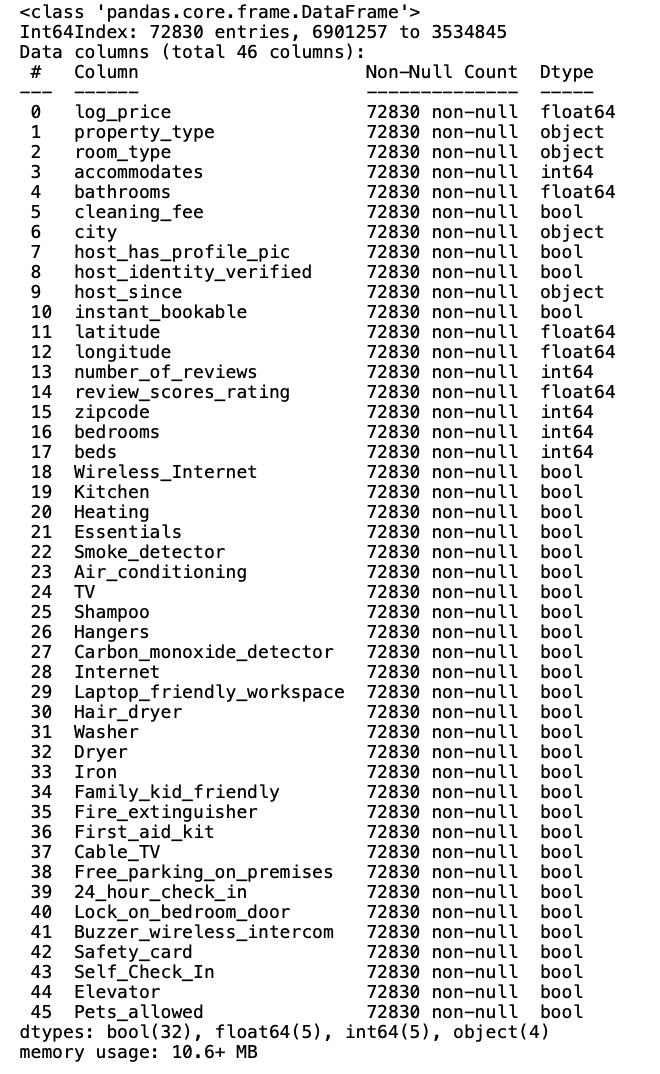
\includegraphics[width=150pt]{info.png}
  \caption{Información del dataset}
\end{figure}


Al confirmar que todo el dataset se encontraba completo se prosiguió con el análisis de cada característica del dataset y su relevancia con el objetivo de proyecto. Como ya se mencionó en secciones pasadas este proyecto tiene como objetivo predecir el precio de reservación en Airbnb de acuerdo con las amenidades que el espacio brinda al cliente. Es por eso que se decidió por eliminar las características relacionadas con el anfitrión del lugar (host\_since, host\_has\_profile\_pic, host\_identity\_verified) las cuales mostraban la fecha de registro del anfitrión, si contaba o no con una foto de perfil y si la identidad del anfitrión ya ha sido verificada. No obstante, es importante mencionar que dichas características serán consideradas para los siguientes análisis y su eliminación se hará al final de estos ya que todavía no se tiene certeza si dichas características tienen una relación relevante con otras características o la característica objetivo (el precio).

Después se pasó a analizar las propiedades intrínsecas de cada característica, esto por medio de estadísticas univariadas, específicamente se seleccionaron las técnicas del umbral de varianza y el coeficiente de correlación de Pearson. 
La varianza es una medida de dispersión que permite saber qué tanto varían una serie de datos respecto a la media aritmética de dicha serie. El objetivo de utilizar la técnica del umbral de varianza es detectar las características constantes y cuasi-constantes, es decir, las características que tienen un valor para todas las instancias o para la casi todas las instancias en el caso de las características cuasi-constantes. Antes de realizar dicha técnica se graficó la distribución de todas las características, esto con el objetivo de tener una visualización de esto. 

\begin{figure}[H]
  \centering
  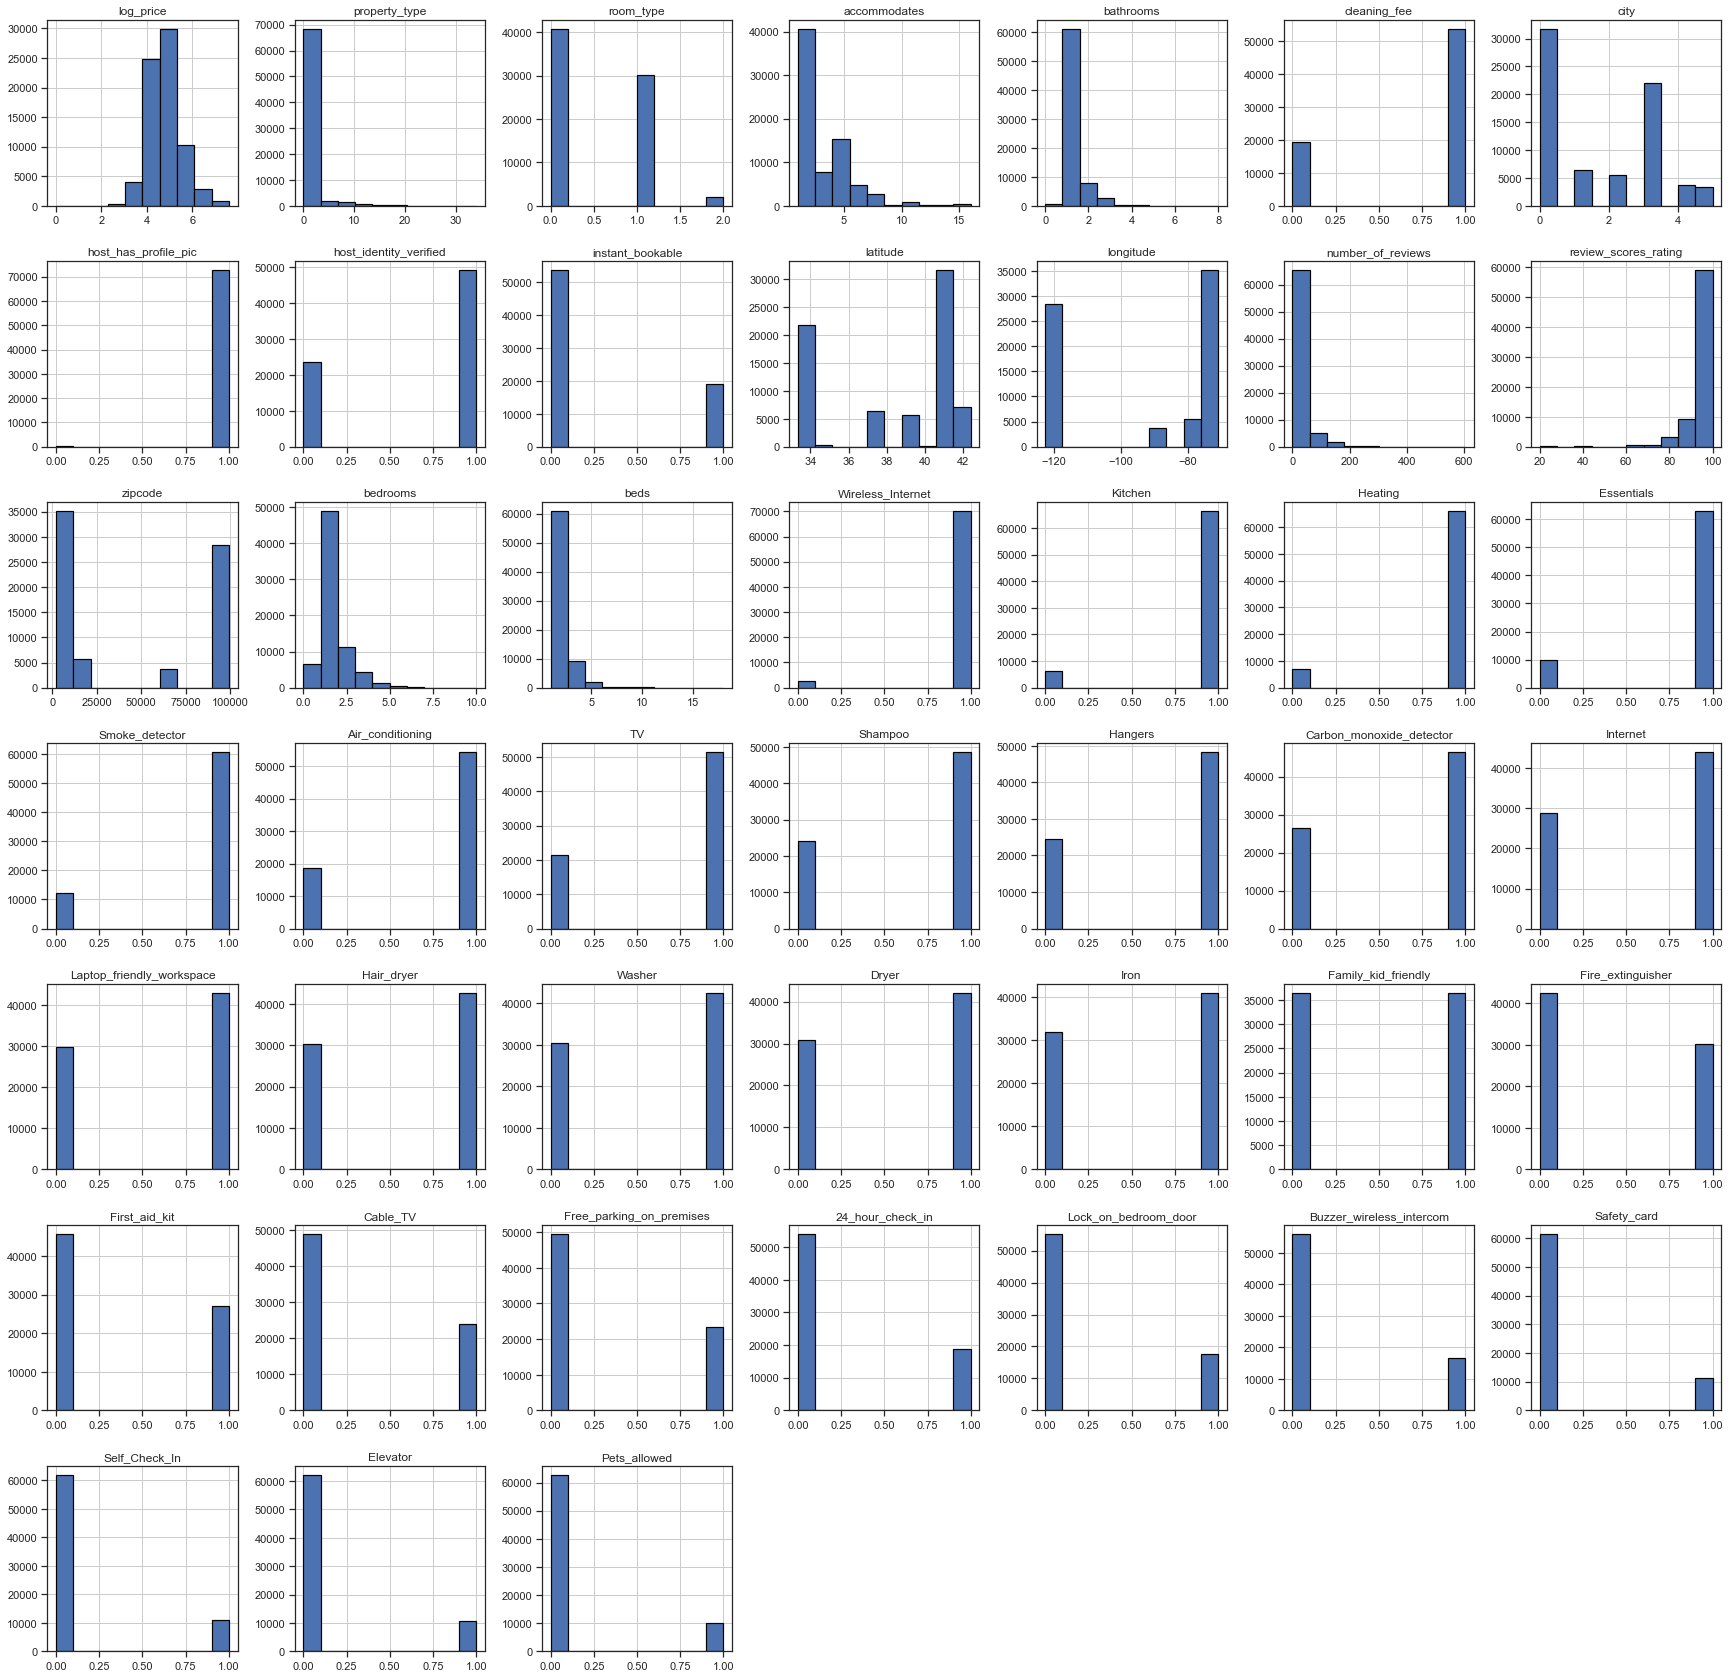
\includegraphics[width=\linewidth]{Distribucion_features.png}
  \caption{Distribuciones de las características}
\end{figure}

Como se puede observar en las gráficas, hay características que tienen una distribución cargada a un valor en específico. Para profundizar más en esto se utilizó la función VarianceThreshold() de la librería scikit-learn con un umbral de 0.05 para detectar así las características que poseen el mismo valor en 95\% o más de sus instancias.

Para algunas columnas, el valor de esas características fue principalmente cero, equivaliendo a un valor false. Esto hace que su varianza sea muy pequeña dejando de añadir información al modelo, es por eso que se tomó la decisión de removerlas del dataset.


\subsection{Limpieza del dataset}
El dataset se encontraba en buen estado, aunque aún así algunas filas tenían valores nulos o inválidos. Para generar un dataset sin irregularidades seguimos los siguientes pasos:

En primer lugar, las columnas con cadenas de caracteres difíciles de analizar (fuera del alcance del proyecto), con demasiados valores irregulares o mal formados, y columnas con valores irrelevantes para el proyecto fueron eliminadas, como:
\begin{itemize}
  \item Tipo de cama
  \item Política de cancelación
  \item Descripción
  \item Fecha de la primera reseña
  \item Tasa de respuesta del anfitrión
  \item Fecha de la última reseña
  \item Nombre de la propiedad
  \item Vecindario en el que se ubica la propiedad
  \item Liga de la imagen de la propiedad
\end{itemize}

Algunas medidas tomadas con filas cuya información podía perjudicar los resultados fueron:
\begin{itemize}
  \item 188 filas fueron eliminadas, ya que no contaban con un valor en la columna "host\_identity\_verified" y en "host\_has\_profile\_pic"
  \item 135 filas que no tenían el número de camas, o que tenían 0 camas fueron eliminadas
  \item 958 filas que tenían un código postal inválido o difícil de analizar fueron eliminadas
  \item Los valores faltantes de la columna "review\_scores\_rating" (promedio de la calificación de las reseñas) fueron completadas con el valor promedio de la columna
  \item Los valores faltantes de las columnas de número de baños y de recámaras fueron llenadas con el valor 0
\end{itemize}

Algunas columnas tenían un tipo de dato incorrecto, por lo que fueron transformadas al tipo de dato que les correspondía, como:
\begin{itemize}
  \item Las columnas 'host\_has\_profile\_pic', 'host\_identity\_verified' y 'instant\_bookable' fueron transformadas a valores booleanos (verdadero si su valor era la cadena "t")
  \item Las columnas "beds" y "bedrooms" fueron transformadas a enteros
  \item Para la columna de código postal, se seleccionaron los primeros 5 caracteres, los cuales fueron utilizados para crear un valor numérico entero
  \item La columna "host\_since" fue convertida al tipo \texttt{pd.DateTime}, que representa una fecha en la librería de Python utilizada para manejar los datos: \texttt{pandas}
\end{itemize}

Otra tarea fue separar la columna de "amenities" en partes, ya que originalmente la columna se encontraba codificada como una lista en JSON (separada por comas, con todas las cadenas entre comillas). La mejor opción para representar esta lista fue hacer una matriz de valores booleanos, en donde cada celda representa si la casa o departamento (fila) contaba con el servicio (columna).

La lista de servicios era muy amplia, por lo que decidimos seleccionar solamente los servicios que tuvieran una frecuencia mayor a 10,000 y que no fueran errores de traducción (un par de servicios empiezan con la leyenda "translation\_missing"), por lo que finalmente se generó una tabla con 28 columnas que representan 28 servicios o permisos:
\begin{itemize}
  \item Wireless\_Internet
  \item Kitchen
  \item Heating
  \item Essentials
  \item Smoke\_detector
  \item Air\_conditioning
  \item TV
  \item Shampoo
  \item Hangers
  \item Carbon\_monoxide\_detector
  \item Internet
  \item Laptop\_friendly\_workspace
  \item Hair\_dryer
  \item Washer
  \item Dryer
  \item Iron
  \item Family\_kid\_friendly
  \item Fire\_extinguisher
  \item First\_aid\_kit
  \item Cable\_TV
  \item Free\_parking\_on\_premises
  \item 24\_hour\_check\_in
  \item Lock\_on\_bedroom\_door
  \item Buzzer\_wireless\_intercom
  \item Safety\_card
  \item Self\_Check\_In
  \item Elevator
  \item Pets\_allowed
\end{itemize}


\subsection{Procesamiento de los datos}
Después de todas las modificaciones que se mencionaron en la secciones anteriores se obtuvo el siguiente dataset: 

\begin{figure}[H]
  \centering
  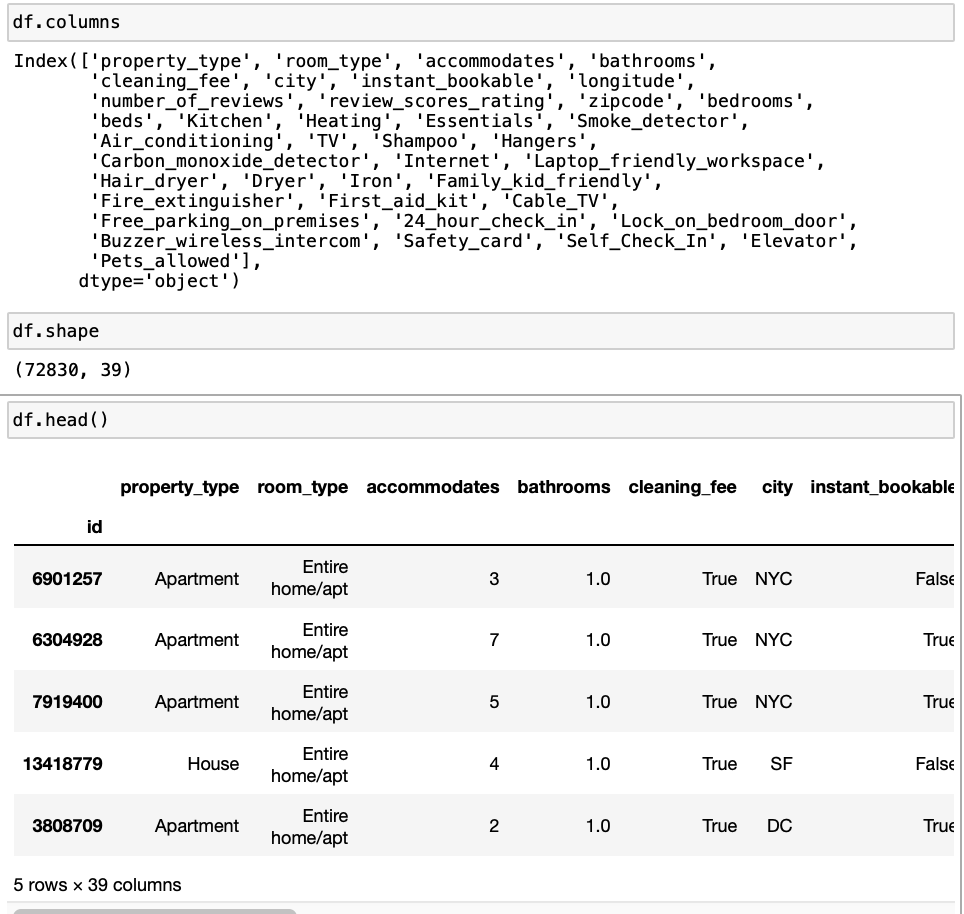
\includegraphics[width=\linewidth]{dataset_actual.png}
  \caption{Distribuciones de las características}
\end{figure}

Como se hizo mención en la sección del análisis estadístico, el dataset contiene en su mayoría características categóricas. Con el fin de facilitar el aprendizaje y reducir el tiempo de ejecución se decidió utilizar un codificador y así hacer que las clases o categorías de cada característica se relacionarán con un valor entero.

Para esto la  librería de scikit-learn propone los codificadores OrdinalEncoder() y OneHotEncoder(). Después de analizar cada uno se optó por usar OneHotEncoder(),  esto principalmente porque OrdinalEncoder() da una jerarquización a los clases o categorías de cada característica y al tener múltiples características con más de dos clases o categorías esto afectaría los resultados esperados sobretodo en los algoritmo que no están hechos en base a árboles de decisiones ya que como se menciona la librería de scikit-learn estos son los que más se ven afectados. 

No obstante, es importante mencionar que una de las desventajas al utilizar el codificador de  OneHotEncoder() es que el tiempo de aprendizaje es más tardado a comparación de OrdinalEncoder(). Esto debido a que OneHotEncoder() hace una matriz de ceros y unos para relacionar todas las clases o categorías de las características y de está manera darle un valor numérico a cada clase o categoría sin hacer una jerarquización. Contrario a lo que hace OrdinalEncoder() que asigna un número de 0 al n-1, siendo n el número de clases. 

Es importante mencionar que se hizo un fit\_transform() para los datos de entrenamiento y transform() para los datos de evaluación, esto por cada iteración.  


\subsection{Modelación}
Posteriormente se declararon las variables "X" y "y", las cuales guardan las características y los precios de las propiedades de Airbnb respectivamente, y se utilizó la función train\_test\_split() para dividir los distintos dataset, logrando obtener el 80\% de los datos para el entrenamiento y el 20\% restante para las pruebas.

Se utilizaron los siguientes modelos de regresión con la ayuda de sklearn\cite{scikit-learn}:
\begin{itemize}
  \item Random Forest Regressor
  \item Gradient Boosting Regressor
  \item Linear Regression
  \item K-Neighbors Regressor
  \item Voting Regressor
\end{itemize}

\subsubsection{Regresión por bosques aleatorios}
Este modelo tomado del módulo sklearn.ensemble consiste en generar particiones aleatorias del set de entrenamiento a través del bootstraping y utilizarlas para entrenar diferentes árboles de decisión para regresión. El modelo toma el promedio de las predicciones resultantes para generar una predicción más estable, evitando el overfitting característico de los árboles de decisión.

\subsubsection{Regresión utilizando Gradient Boosting}
Este modelo también pertenece al módulo sklearn.ensemble.
Su finalidad es minimizar una función de error que puede ser especificada\cite{draper1998applied}, la opción escogida fue la de error cuadrático medio, que viene por defecto.

$$MSE = \frac{1}{n} \sum_{i=1}^{n} (y_i - \hat{y})$$

En el caso de esta implementación, el modelo usa árboles de decisión para poder realizar las regresiones.
Los parámetros importantes como learning rate o criterio se dejaron como los valores por defecto.

\subsubsection{Regresión lineal}
El modelo de regresión lineal se basa en la ecuación que define la línea recta para establecer una predicción.

$$y = X\vec{B} + \epsilon$$

El parámetro fit:intercept se cambió al valor "True", mientras que todos los demás parámetros se dejaron con sus valores por defecto.

\subsubsection{Regresión utilizando k-Vecinos más cercanos}
El modelo de regresión basado en K-Neighbors realiza una predicción obteniendo el promedio de los valores de los vecinos más cercanos.

En este caso el número de vecinos utilizados fue 30. El parámetro n\_jobs se definió como -1 para permitir que se utilicen todos los núcleos del cpu en el proceso.

\subsubsection{Regresión utilizando un algoritmo de votación}
Este modelo permite establecer una predicción obteniendo el promedio de las predicciones de varios modelos, todos aplicados a un mismo set de datos.
Al igual que el modelo de K-neighbors el parámetro n\_jobs se inicializó como -1.
Con la finalidad de obtener una predicción que tomara en cuenta los resultados previos, para este modelo se utilizaron los modelos ya mencionados.


\section{Resultados}
Todos los modelos se ejecutaron 28 veces, con un for loop y procurando que el parámetro de random\_state de train\_test\_split fuera siempre el número de iteración. Esto para garantizar que cada iteración mostrara un resultado diferente por iteración pero repetible cada que se corra el programa.

Se inicializaron cinco arrays vacíos antes del ciclo for para que con cada iteración las puntuaciones de cada modelo se fueran guardando en sus respectivos arreglos. Al terminar el ciclo todos los arrays son guardados como csv en la misma carpeta donde el programa se encuentra.

Por último, se grafican los datos reales junto con la predicción de cada modelo para las primeras diez instancias, esto para poder visualizar el comportamiento de los modelos.

\begin{figure}[H]
  \centering
  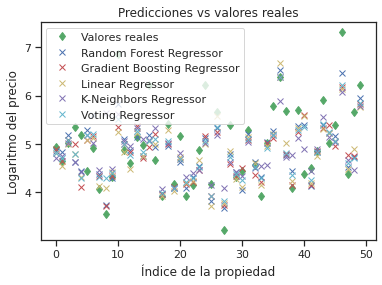
\includegraphics[width=\linewidth]{grafica_resultados.png}
\end{figure}

Los resultados para el error cuadrático medio obtenidos para los modelos en una sola iteración fueron los siguientes:

\begin{table}[]
\begin{tabular}{|c|c|}
\hline
\textbf{Modelo}           & \textbf{MSE} \\ \hline
\textbf{RandomForest}     & 0.16103      \\ \hline
\textbf{GradientBoosting} & 0.17754      \\ \hline
\textbf{LinearRegression} & 0.16551      \\ \hline
\textbf{KNeighbors}       & 0.22458      \\ \hline
\textbf{VotingRegressor}  & 0.15988      \\ \hline
\end{tabular}
\end{table}

\subsection{Prueba de Wilcoxon}
Se realizó la prueba de Wilcoxon a los 22 resultados de MSE para cada modelo. Los resultados totales se pueden encontrar en el apéndice C, pero en resumen, el ranking de modelos fue en este orden:
\begin{enumerate}
  \item Voting Regressor
  \item Random Forest Regressor
  \item Linear Regression
  \item Gradient Boosting
  \item K-Neighbors
\end{enumerate}

\section{Conclusiones}
No es un resultado fuera de lo común, tomando en cuenta el funcionamiento del Voting Regressor y el Random Forest, los cuales toman en cuenta las predicciones de distintas modelos únicos, con diferentes sesgos.

A pesar de esto, resulta interesante que el modelo de regresión lineal haya resultado estadísticamente mejor que los modelos de gradient boosting y KNeighbors regressor.


\bibliographystyle{ACM-Reference-Format}
\bibliography{references}

\clearpage

\appendix

\begin{figure*}
  \section{Código para la comparación de modelos de regresión}
  \label{appendix:regs}
  \inputminted[lastline=60]{python}{/home/mario/git/MarioJim/AirbnbPricePrediction/generate_mses_updated.py}
\end{figure*}

\begin{figure*}
  \section{Código de prueba de Wilcoxon}
  \label{appendix:wilc}
  \inputminted{python}{/home/mario/git/MarioJim/AirbnbPricePrediction/wilcoxon_test.py}
\end{figure*}

\begin{figure*}
\section{Salida de ejecución de prueba de Wilcoxon}
\label{appendix:wilc_out}

\subsection{Wilcoxon rank sums test with a greater hypothesis}
\begin{tabular}{|c|c|c|c|c|c|}
\hline
\textbf{}                 & \textbf{GradientBoosting} & \textbf{KNeighbors} & \textbf{LinearRegression} & \textbf{RandomForest} & \textbf{VotingRegressor} \\ \hline
\textbf{GradientBoosting} & 0.5                       & 0.00000000671996    & 0.99999999328004          & 0.99999999328004      & 0.99999999328004         \\ \hline
\textbf{KNeighbors}       & 0.99999999328004          & 0.5                 & 0.99999999328004          & 0.99999999328004      & 0.99999999328004         \\ \hline
\textbf{LinearRegression} & 0.00000000671996          & 0.00000000671996    & 0.5                       & 0.99819635515675      & 0.99999850169938         \\ \hline
\textbf{RandomForest}     & 0.00000000671996          & 0.00000000671996    & 0.00180364484325          & 0.5                   & 0.99698639393373         \\ \hline
\textbf{VotingRegressor}  & 0.00000000671996          & 0.00000000671996    & 0.00000000001436          & 0.00301360606627      & 0.5                      \\ \hline
\end{tabular}

\subsection{Wilcoxon rank sums test with a less hypothesis}
\begin{tabular}{|c|c|c|c|c|c|}
\hline
\textbf{}                 & \textbf{GradientBoosting} & \textbf{KNeighbors} & \textbf{LinearRegression} & \textbf{RandomForest} & \textbf{VotingRegressor} \\ \hline
\textbf{GradientBoosting} & 0.5                       & 0.00000000671996    & 0.99999999328004          & 0.99999999328004      & 0.99999999328004         \\ \hline
\textbf{KNeighbors}       & 0.99999999328004          & 0.5                 & 0.99999999328004          & 0.99999999328004      & 0.99999999328004         \\ \hline
\textbf{LinearRegression} & 0.00000000671996          & 0.00000000671996    & 0.5                       & 0.99819635515675      & 0.99999850169938         \\ \hline
\textbf{RandomForest}     & 0.00000000671996          & 0.00000000671996    & 0.00180364484325          & 0.5                   & 0.99698639393373         \\ \hline
\textbf{VotingRegressor}  & 0.00000000671996          & 0.00000000671996    & 0.00000000001436          & 0.00301360606627      & 0.5                      \\ \hline
\end{tabular}

\end{figure*}

\begin{figure*}
  \section{Mapa de correlación entre variables}
  \begin{figure}[H]
    \centering
    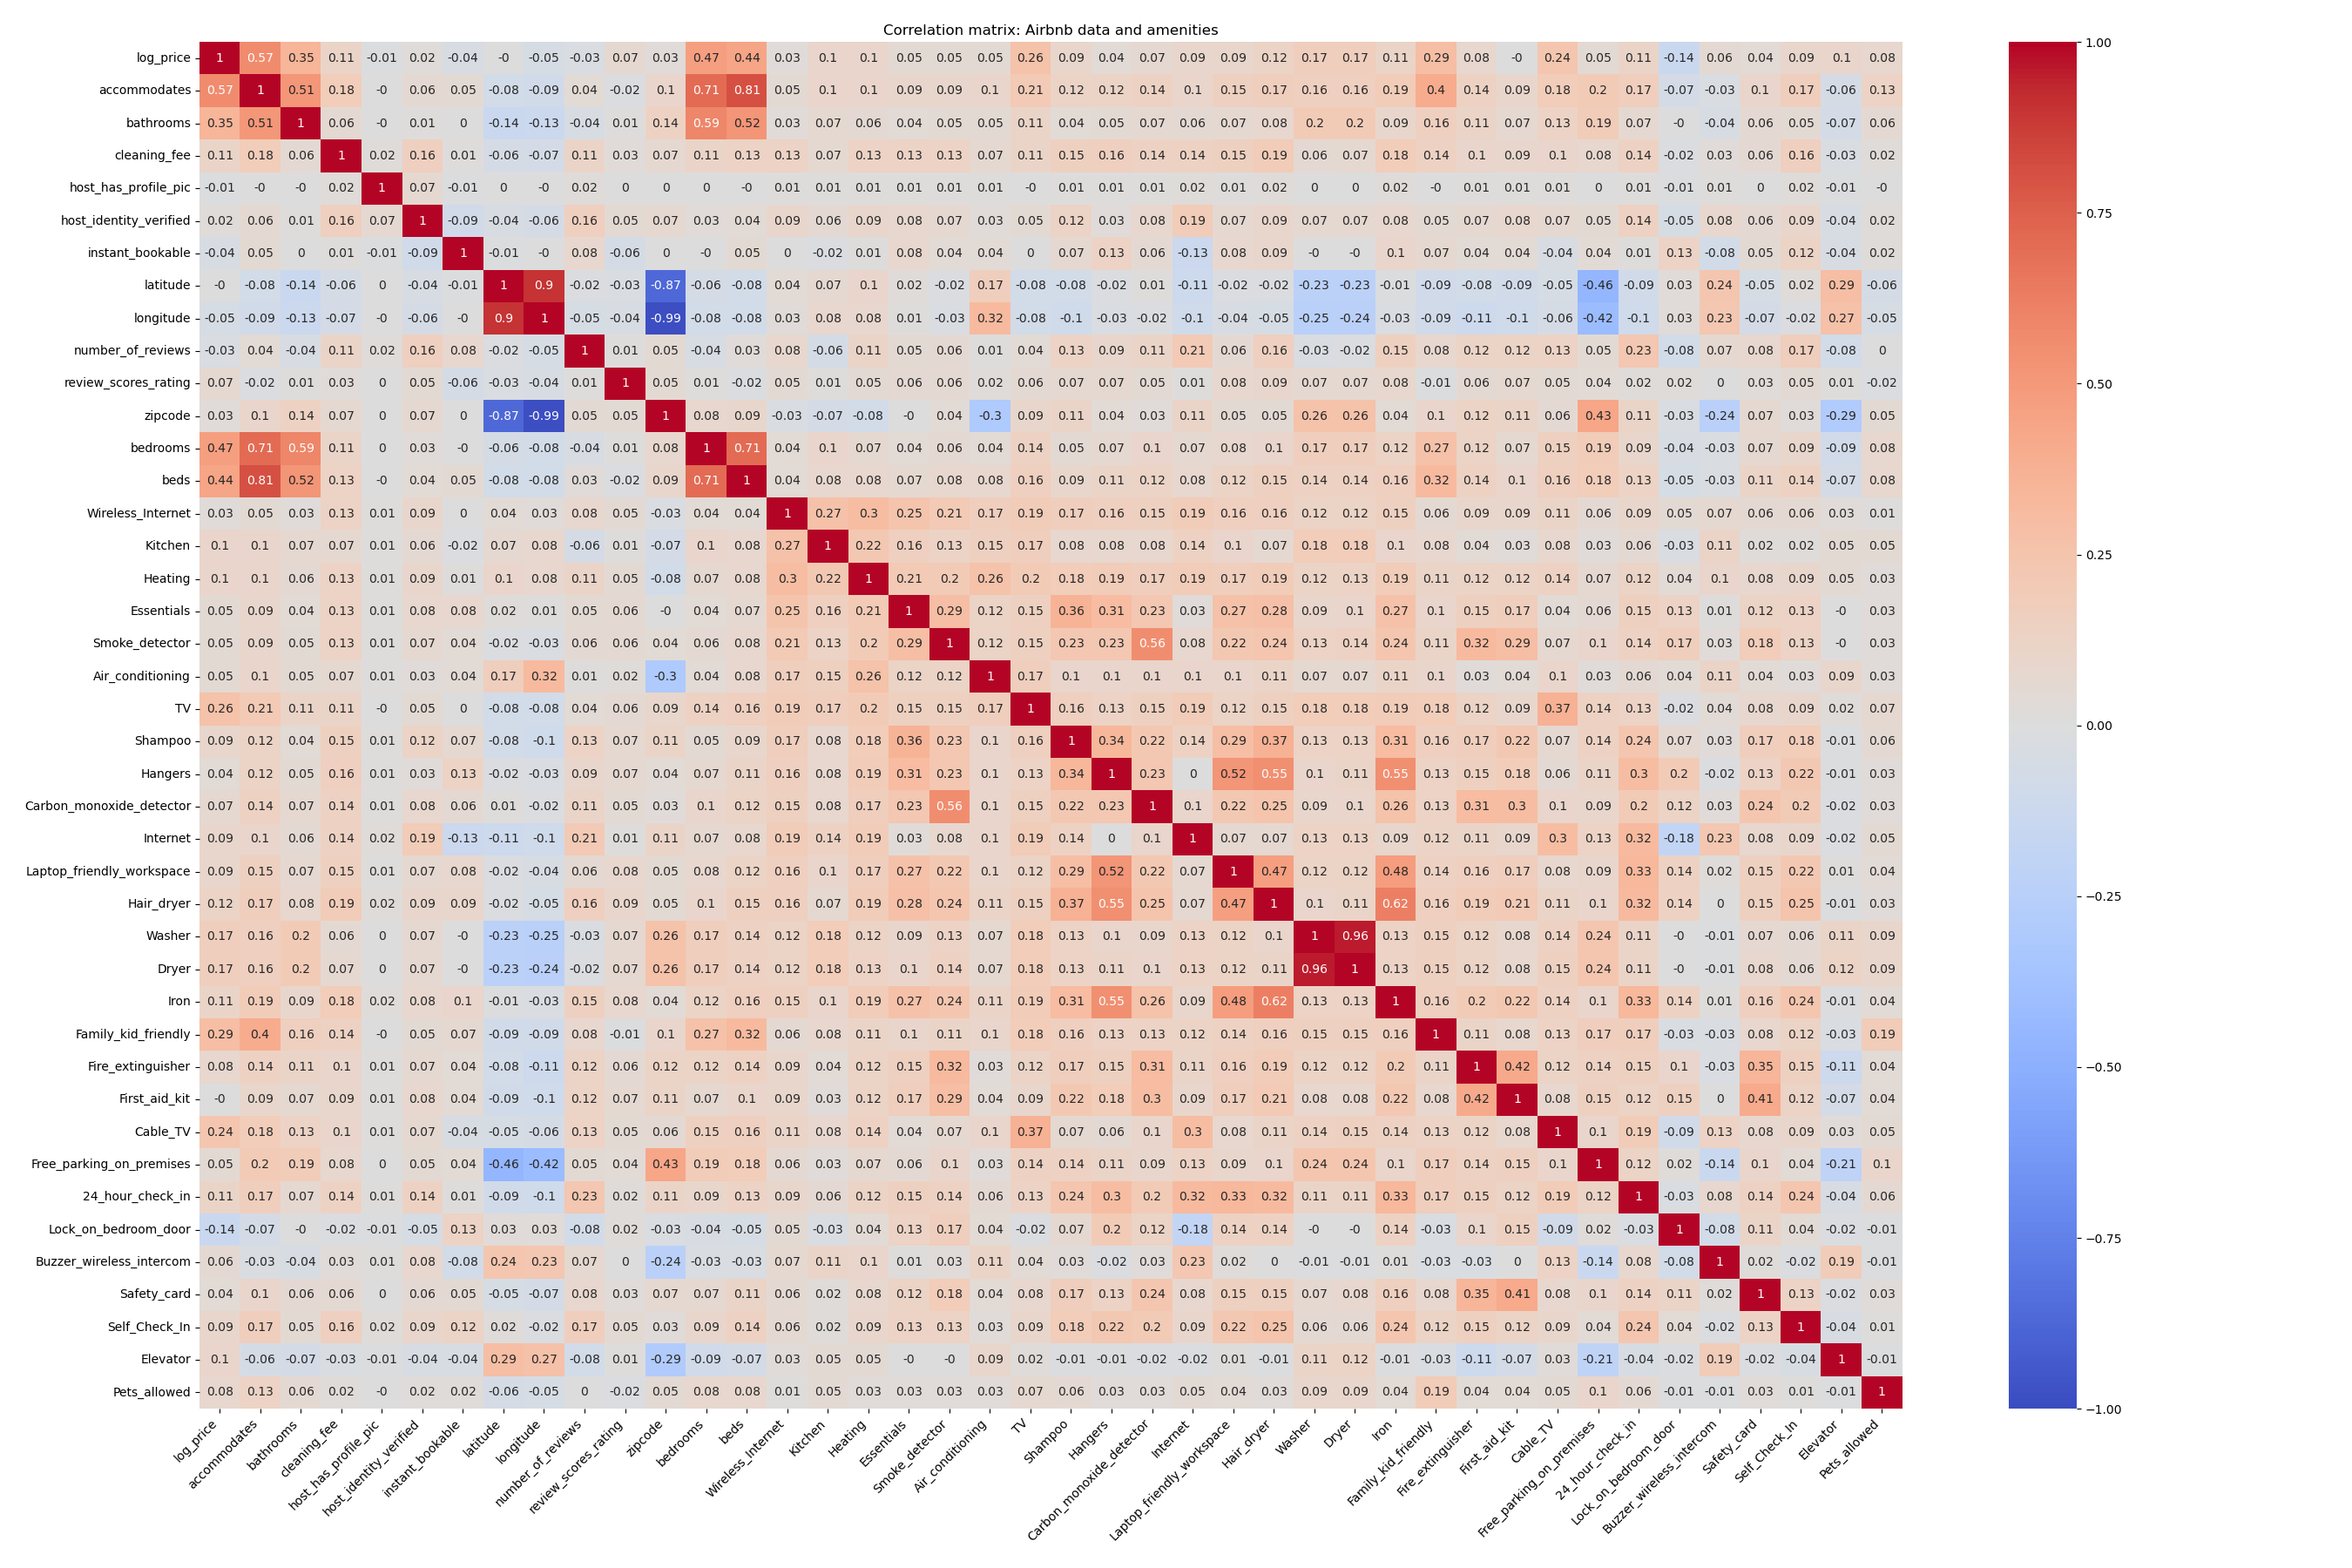
\includegraphics[width=500pt]{corrmtx_concat.png}
  \end{figure}
\end{figure*}

\end{document}
\endinput
